\chapter {Experiments}

The algorithms as described above, is tested on three hypothetical problem instances. Description of all
the problem instances is defined in the next section. Two real life problem instances, Ajmer and Konkan 
railways still need to be tested but the hypothetical problem instances are comparable in size 
to the real life instances. Code for whole implementation is at \cite{WEBSITE:6}.

\section {Problem Instances}
\subsection{HYP-1}
The simple hypothetical instance HYP-1 consists of 8 trains
travelling 5 stations each. All trains are already
in the system at the start. Four trains heading left to right are
initially located in station Alpha, while the
others are in station Echo, heading right to left. Each station
contains 4 parallel tracks, and there is a single track between
stations. Only for HYP-1, the trains all have the same priority,
running times between stations, and halt times at stations.

\begin{figure}[h]
    \centering
    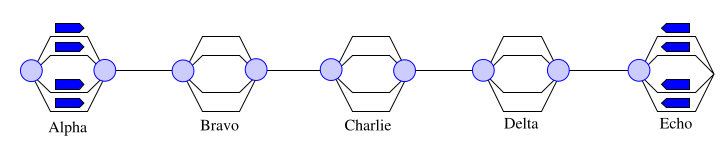
\includegraphics[width=0.7\textwidth]{Instance1}
    \caption{ HYP-1 \cite{ARTICLE:1} }
    \label{Instance1}
\end{figure}

\subsection{HYP-2 \& HYP-3}
HYP-2 have 11 stations each having 3 tracks and each station is connected by a single bidirectional track.
The scheduling problem starts from the clean slate i.e. initially no train is in the network.
HYP-2 have 60 trains, 40 priority-1 train and 20 priority-2 train running. HYP-3 have double the number of trains 
i.e. 120 trains with 80 priority-1 train and 40 priority-2 train. Since the number of trains have 
doubled up, in HYP-3 each station have 4 tracks and single track is connecting these stations.

\begin{table}[H]
    \centering
    \caption{Hypothetical instances}
    \label{Dataset}
    \begin{tabular}{ c c c c  } 
     \hline
     \textbf{Name} & \textbf{Stns.} & \textbf{Trains (sorted by priority)} & \textbf{Events} \\ 
     \hline
     \hline
     HYP-1 & 5 & 8,0,0 & 40 \\
    
     HYP-2 & 11 & 15,45,0 & 1320 \\
     
     HYP-3 & 11 & 40,80,0 & 2640 \\ 
     \hline
    \end{tabular}
\end{table}

\section{Hyperparameters}
All results use a look-forward of $l_f = 6$ resources, and a
look-back of $l_b = 2$ resources. The status of each resource
takes one of three values: 0, 1, or 2 ($R = 3$). The weight on
converging trains is $w_c = 0.9$, while that on diverging trains
is $w_d = 1$. The maximum number of priority levels is $P = 3$.
In case of modified $\epsilon$ - greedy policy, the threshold for checking whether $q_0 \approx q_1$ 
is $\tau = 0.9$, and the aggression parameter is $\alpha = 0.9$. The
threshold for determining the maximum acceptable J is
$\rho = 0.25$. In case of Sarsa($\lambda$) , $\lambda = 0.9$ is choosen.

\vspace{\baselineskip}
Training is run for 500 episodes, where the $\epsilon$ is linearly reduced from 1 to 0.1 in 300 
episodes. Note, that the value of $\epsilon$ remains the same in each episode. Decrease in the value of 
$\epsilon$ is per episode basis.

\section {Results}
\subsection{Sarsa ($\lambda$) on HYP-1}

\begin{figure}[h]
    \centering
    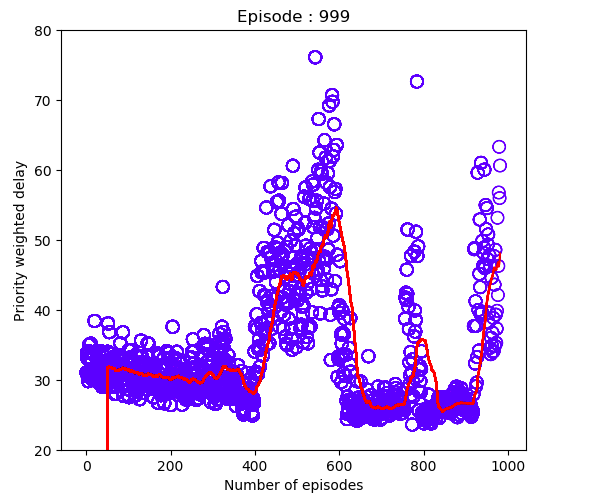
\includegraphics[width=0.7\textwidth]{Sarsa_HYP-1}
    \caption{ Priority weighted delay for Sarsa($\lambda$) on HYP-1 over 1000 episodes training}
    \label{Sarsa_HYP-1}
\end{figure}

Sarsa($\lambda$) is not able to find an optimal schedule even for HYP-1. In the above plot, 
blue dots are the delay for one training episode, while red line is the running mean over the 
last 50 episodes.
The results of this algorithm is not good (in the next section) due to following reasons,
\begin{enumerate}
\item The back-propagation of rewards
      after the end of the episode is not possible, because the episode
can be very long.
\item In the trajecotry of a train, it is possible to visit the same state-action pair in loop leading to 
large accumulation of reward at that state-action pair, leading to extreme values.
\item Moreover, the magnitude of delays (and hence the theoretical
optimum value of $J$ ) is different from one problem instance
to another. Quantifying rewards directly in terms of delays
$\delta_{r,t}$ would create obstacles when transferring the learning from
one instance to another (\textbf{obstacle in transfer learning}).
\end{enumerate}

\subsection{Proposed work on HYP-1}
Q-values are initialised to 0.5 as they in some sense represent the probability of taking action either 
to move or to wait.
Training on the HYP-1 using the proposed approach, results in the convergence of Q-values. The Q-values 
decreased from around 35 to around 25. \textbf{Minimum is 23.58750}. Note the delay is only for those episodes that 
are successfully completed (not ending up in deadlock). Total number of episodes that ended up in deadlock 
are only 3 out of 500 episodes.

\begin{figure}[H]
    \centering
    \includegraphics[width=0.7\textwidth]{/home/arpit/study/BTP/Results_image/HYP1/Approach2/1/delay}
    \caption{ Priority weighted delay for proposed approach on HYP-1 over 500 episodes training }
    \label{HYP-1_Approach2_delay}
\end{figure}

The figure \ref{Schedule_HYP-1}, shows time on the x-axis and
distance on the y-axis. Each solid line shows the trajectory of 
one train as it moves from one end of the line to the other. The
horizontal portions correspond to halts at stations, while the
inclined portions denote movement between stations. Since
there is a single track between successive stations and only
one train can occupy it at a time, inclined lines cannot cross
each other in a feasible schedule. The horizontal dotted lines
indicate specific tracks within station resources, and no two
solid lines are allowed to overlap within these tracks.

\begin{figure}[H]
    \centering
    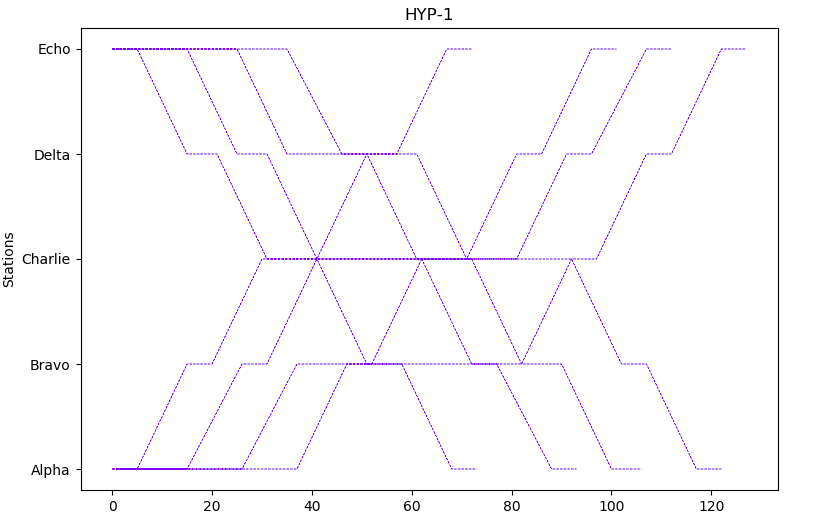
\includegraphics[width=0.7\textwidth]{/home/arpit/study/BTP/Results_image/HYP1/Approach2/1/train_running}
    \caption{ Schedule computed using proposed approach for HYP-1}
    \label{Schedule_HYP-1}
\end{figure}

\section{Training on HYP-2 \& HYP-3}
The toy instance like HYP-1 shows that the proposed
approach is able to learn Q-Values (and hence the policy for
choosing actions) at a small scale. However, when instances
of a realistic size and complexity are run with the same
initial Q-Values (0.5\%), they require a large number of training
instances to start producing feasible solutions. This happens
because the larger problem instances require several thousand
decisions to be made ‘correctly’ for successful completion.
When such decisions are made purely randomly, the instances
frequently end with trains in deadlock situations. 
So in order to speed up the training, the Q-values are initialized according to heuristic \ref{Heuristic}.

\begin{table}[H]
    \centering
    \caption{\textbf{Heuristic For initialising Q-values}}
    \label{Heuristic}
    \begin{tabular}{ c c c c  } 
     \hline
     \textbf{\#} & \textbf{States Satisfying} & \textbf{Action} & \textbf{Init Q-values} \\ 
     \hline
     \hline
    1 & Next Resource is Full & Move & 0 \\
     & $ S_{r,next} = R-1 $ & Stop & 50\\
    
     2 & Atleast three consecutive resources are full & Move & 10 \\
     & $ S_r = S_{r+1} = S_{r+2} = R-1 $   & Stop & 15\\
    
     3 & Next Resource almost Full (R-2) & Move & 15 \\
     & Next but one is full (R-1) & Stop & 50 \\
    
     4 & Average status of upcoming resources & Move & 85 \\
     & is between 0.5 and 1.0 (moderately empty) & Stop & 90\\
     
     5 & Average status of upcoming resources & Move & 95 \\
      & is less than 0.25 (almost empty)  & Stop & 50\\
     \hline

    \end{tabular}
\end{table}

Training over different problem instances is summarized by table \ref{Training}. First row corresponds to training 
using prior Q-value while second row corresponds to proposed Q-value .  Second column shows the
minimum objective function attained during training, third column shows number of episodes ending 
in deadlock out of 500 training episodes and fourth column shows the total number of 
episodes visited out of $3 * 3^{2 + 1 + 6}  = 59049$ states. Table \ref{Training}, shows HYP-3 is the most extensive problem 
instance visiting large number of states, so can be ideally most suitable for transfer learning.

\begin{table}
    \centering
    \caption{\textbf{Training}}
    \label{Training}    
        \begin{tabular}{  c c c c c } 
         \hline
         \textbf{Instance} & \textbf{Minimum} & \textbf{Deadlock} & \textbf{Total states visited} \\ 
         \hline
         \hline
         HYP-1 & 23.53750 & 3 & 354 \\
         & 23.58750 & 3 & 348 \\
     
         HYP-2 & 2.60682 & 3 & 1650 \\
         & 2.58447 & 5 & 1712 \\
     
         HYP-3 & 11.64754 & 32 & 3377 \\
         & 11.34754 & 29 & 3021 \\
         \hline

        \end{tabular}
\end{table}
    

Training on HYP-3 is able to converge from 25 to almost 12 with 11.34754 as the minimum objective 
value. Red curve in the plot is the running mean over the last 50 episodes. In the figure \ref{deadlock_HYP-3}, ratio of 
episodes ended in deadlock as the training progresses is shown. It can be clearly seen, as the training 
progresses, percentage of episodes ending in deadlock starts to decrease with almost 25\% in 100 episodes 
to almost 5\% in 500 episodes. This shows that the algortihm learns to avoid deadlock as the training progresses. 

\vspace{\baselineskip}
Figure \ref{Schedule_HYP-3}, shows the schedule generated for HYP-3. The plot shows the density and complexity of the 
schedule generated for the trains running over the HYP-3 network. Blue dashed line shows the trajectory of 
priority-1 train while red dashed line shows the trajectory of priority-2 trains.


\begin{figure}[H]
    \centering
    \includegraphics[width=0.7\textwidth]{/home/arpit/study/BTP/Results_image/HYP3/Approach2/1/delay}
    \caption{ Objective function for training over HYP-3 }
    \label{delay_HYP-3}
\end{figure}
\begin{figure}[H]
    \centering
    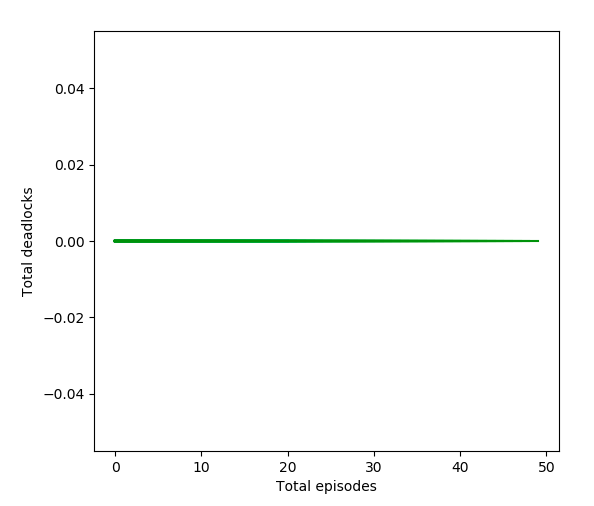
\includegraphics[width=0.7\textwidth]{/home/arpit/study/BTP/Results_image/HYP3/Approach2/1/deadlock}
    \caption{ Deadlock in \% for training over number of episodes in HYP-3 }
    \label{deadlock_HYP-3}
\end{figure}
\begin{figure}[H]
    \centering
    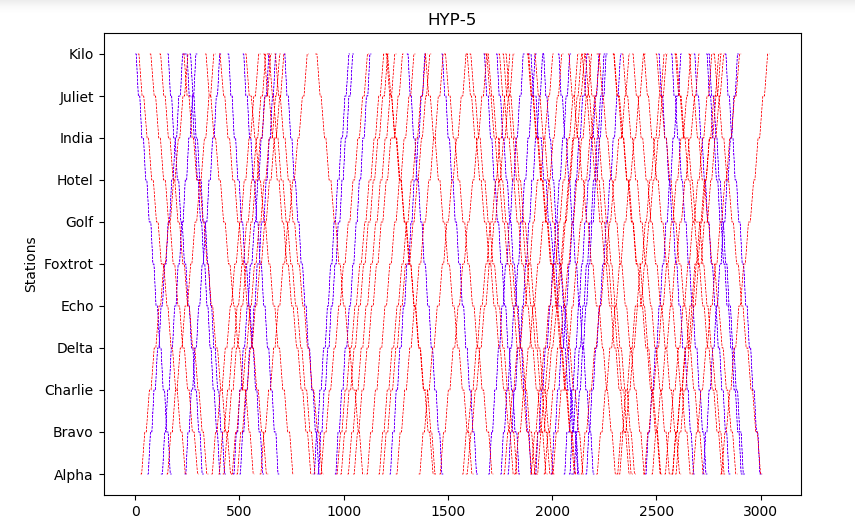
\includegraphics[width=0.9\textwidth]{/home/arpit/study/BTP/Results_image/HYP3/Approach2/1/running_train}
    \caption{ Schedule computed using proposed approach on HYP-3 with blue line for priority-1 train 
              and red line for priority-2 train. }
    \label{Schedule_HYP-3}
\end{figure}
\section{Testing and transfer learning}

This section summarises the result of testing and transfer learning (training on one problem instance 
and testing on other problem instance).Testing is done over \textbf{50 episodes}.
Two types of testing are done,
\begin{enumerate}
    \item \textbf{Zero Delay} : No external delay is introduced in the system.
    \item \textbf{20\% Delay} : Delay of 20\% is introduced in the system. Delay is introduced by 
                                randomly increasing the running time between two consecutive stations. 
                                20\% means that running time almost shoots by 20\%. Note delay is introduced in 
                                the whole network uniformly. In future, delay can be introduced only in section of the 
                                network.
\end{enumerate}
Following table summarizes the results of testing. First row shows the results for prior work while 
second row shows the results for proposed work . It is clear from results that proposed Q-value works better
compared to proposed one.

\vspace{2in}

\begin{table}[H]
\centering
\caption{\textbf{Zero delay}}    
    \begin{tabular}{ c c c c c } 
     \hline
     \textbf{Train} & \textbf{Test} & \textbf{Minimum} & \textbf{Average} & \textbf{deadlock} \\ 
     \hline
     \hline
     HYP-2 & HYP-2 & 4.050 & 4.980 $\pm$ 0.590 & 0 \\
     & & \textbf{2.680} & \textbf{3.257 $\pm$ 0.501} & \textbf{0} \\
    
     HYP-3 & HYP-2 & 3.089 & \textbf{4.080 $\pm$ 0.370} & 0 \\
     & & \textbf{2.709} & 4.184 $\pm$ 0.438 & \textbf{0} \\
    
     HYP-2 & HYP-3 & 12.683 & 14.580 $\pm$ 1.058 & 16 \\
     & & \textbf{11.453} & \textbf{13.083 $\pm$ 1.164} & \textbf{6} \\
    

     HYP-3 & HYP-3 & 11.855 & 12.954 $\pm$ 0.540 & 1 \\
     & & \textbf{11.438} & \textbf{12.734 $\pm$ 0.613} & \textbf{0} \\
     \hline
    \end{tabular}
\end{table}


\begin{table}[H]
    \centering
    \caption{\textbf{20\% delay}}    
        \begin{tabular}{ c c c c c } 
         \hline
         \textbf{Train} & \textbf{Test} & \textbf{Minimum} & \textbf{Average} & \textbf{deadlock} \\
         \hline
         \hline
         HYP-2 & HYP-2 & 9.591 & 11.388 $\pm$ 1.258 & \textbf{0} \\
         & & \textbf{8.386} & \textbf{10.261 $\pm$ 0.733} & 1 \\
     
         HYP-3 & HYP-2 & 9.603 & 10.932 $\pm$ 0.881 & 3 \\
         & & \textbf{8.473} & \textbf{10.472 $\pm$ 0.792} & \textbf{1} \\
     
         HYP-2 & HYP-3 & \textbf{26.882} & 31.955 $\pm$ 2.290 & \textbf{23} \\
         & & 27.734 & \textbf{30.141 $\pm$ 1.486} & 29 \\
     
         HYP-3 & HYP-3 & \textbf{26.522} & 30.135 $\pm$ 1.649 & 3 \\
         & & 26.560 & \textbf{29.231 $\pm$ 1.723} & \textbf{1} \\
        \hline
        \end{tabular}
\end{table}

In future, we are planning to test on real life datasets like ajmer and konkan railway lines. Delay can be 
introduced only in some part of the network to check the robustness of the algorithm. Moreover, testing on railway
network (with atleast one intersection of railway lines) is also to be done. However it is very less likely that the 
given algorithm performs good over those instances as the state space is defined in view of only the railway line.
More robust state space (observation) in case of railway networks is \textbf{tree like observations} which is the 
future work.

